\chapter{Joint topography correction and reconstruction}\label{ch:joint}

The analysis of \cref{sec:sata-limit} shows that the correct phase (the $\dC$ read from the DEM) is already known; what
fails is applying it per channel before the parcels are separated. The joint reconstruction moves the DEM phase inside the
inversion.

\section{Joint reconstruction in the sub-apertures}

With the same sub-apertures as SATA, for every sub-aperture and every bin $\phi$ of the $\Nrx$ channel spectra the model
\eqref{eq:fold} is written with the phase of each parcel at its own ground position:
\begin{equation}
  S_i(\phi) = \sum_q H_i(f_q)\,\exp\!\Bigl(-\jj\frac{2\pi}{\lambda}\Delta C_{0,i}(x_q)\Bigr)\,U_q,
  \qquad x_q = x_c + \frac{\lambda r_0}{2v} f_q ,
\end{equation}
and solved for the parcels $U_q$, which are then placed at their true Doppler, transformed back and overlap-added at the
full PRF. The steps are summarised in \cref{fig:flowsubap}. With $\dC=0$ this is the standard reconstruction ($\sim10^{-7}$); with one target it
equals the oracle. Its limit is the resolution of the sub-aperture: the DEM is read once per bin of a \SI{40}{ms} block, i.e.\
the terrain phase is taken as constant over about $\pm\SI{600}{m}$ of ground. A slope $s$ with a cross-track baseline is
equivalent to shifting the phase centre of the channel by $\bxt s/(2\tan\theta)$; when that shift is not small compared with
the block, the per-bin model breaks. With $\Delta\varphi=\frac{2\pi}{\lambda}\,\frac{\bxt^{\max}\,s\,\delta x}{r_0\tan\theta}$
the phase change inside one SATA cell, the method stays within about \SI{10}{dB} of the reference for
$\Delta\varphi\lesssim\SI{0.5}{rad}$ and fails by 10 to \SI{35}{dB} above \SI{1}{rad}.

\begin{figure}[p]
\centering
% Flowchart of the joint reconstruction in the sub-apertures (reconstruct_joint)
\begin{tikzpicture}[x=1cm,y=1cm,node distance=4mm]
  \node[bdata,text width=62mm] (in) at (0,0) {\textbf{Inputs}: channels $s_i[m]$ at $\PRFop$, DEM $h(x)$, geometry};
  \node[bprep,below=5mm of in,text width=62mm] (p1) {reference-point filters\\ $(C_0,C_1,C_2,\Delta t)\to H_i(f)$};
  \node[bprep,below=2.5mm of p1,text width=62mm] (p2) {DEM table: $\Delta C_{0,i}$ at every cell};
  \node[bprep,below=2.5mm of p2,text width=62mm] (p3) {block grid (20 samples, hop 10, FFT of 128),\\ parcel frequencies $f_q(\phi)$, ruler $x(f)$};
  \node[bloop,below=5mm of p3,text width=62mm] (b1) {block $k$: triangular window + zero padding};
  \node[bloop,below=2.5mm of b1,text width=62mm] (b2) {FFT of every channel $\to S_i(k,\phi)$};
  \node[bloop,below=2.5mm of b2,text width=62mm] (b3) {ruler: position $x_q(\phi)$ of every parcel\\ $\to$ read $\Delta C_{0,i}(x_q)$ in the DEM table};
  \node[bloop,below=2.5mm of b3,text width=62mm] (b4) {matrix of the bin\\ $G_{iq}=H_i(f_q)\,\e^{-\jj2\pi\Delta C_{0,i}(x_q)/\lambda}$};
  \node[bloop,below=2.5mm of b4,text width=62mm] (b5) {least squares for the parcels:\\ $\hat{\bm u}(\phi)=\mathbf G^{+}\bm S(\phi)$};
  \node[bloop,below=2.5mm of b5,text width=62mm] (b6) {parcels at their true Doppler (full band)\\ $\to$ IFFT at the full PRF};
  \node[bloop,below=2.5mm of b6,text width=62mm] (b7) {overlap-add + sum of the windows};
  \node[bdec,below=4mm of b7] (dec) {last\\ block?};
  \node[bfin,below=4mm of dec,text width=62mm] (f1) {normalise by the sum of the windows};
  \node[bfin,below=2.5mm of f1,text width=62mm] (f2) {limit to the band $\Ba$};
  \node[bdata,below=4mm of f2,text width=62mm] (out) {full-rate line, in the form of\\ the standard reconstruction};
  \foreach \a/\b in {in/p1,p1/p2,p2/p3,p3/b1,b1/b2,b2/b3,b3/b4,b4/b5,b5/b6,b6/b7,b7/dec,f1/f2,f2/out}{\draw[seta] (\a) -- (\b);}
  \draw[seta] (dec) -- node[right,nota]{yes} (f1);
  \node[blk,right=12mm of b4,text width=22mm] (nx) {$k\leftarrow k+1$\\ (hop of 10\\ samples)};
  \draw[seta] (dec.east) -| node[pos=0.2,above,nota]{no} (nx.south);
  \draw[seta] (nx.north) |- (b1.east);
  \foreach \n/\l in {p1/P1,p2/P2,p3/P3,b1/B1,b2/B2,b3/B3,b4/B4,b5/B5,b6/B6,b7/B7,f1/F1,f2/F2}{
     \node[stepn] at ($(\n.west)+(-0.45,0)$) {\l};}
  \draw[decorate,decoration={brace,amplitude=5pt,mirror},inkb] ($(p1.north west)+(-0.95,0.05)$) -- node[left=6pt,nota]{once} ($(p3.south west)+(-0.95,-0.05)$);
  \draw[decorate,decoration={brace,amplitude=5pt,mirror},inkb] ($(b1.north west)+(-0.95,0.05)$) -- node[left=6pt,nota]{every\\ block} ($(b7.south west)+(-0.95,-0.05)$);
  \draw[decorate,decoration={brace,amplitude=5pt,mirror},inkb] ($(f1.north west)+(-0.95,0.05)$) -- node[left=6pt,nota]{once} ($(f2.south west)+(-0.95,-0.05)$);
  \node[nota,anchor=west] at ($(b5.east)+(0.3,0)$) {for each of\\ the 128 bins};
\end{tikzpicture}

\caption[Flowchart of the joint reconstruction in the sub-apertures]{The joint reconstruction in the sub-apertures. Green: preparation, done once. Blue: the loop over the blocks of 20 samples; inside each block a small
least-squares system is solved for every bin. Violet: finishing. The DEM is read once per bin, at the position the ruler gives to
each parcel.}
\label{fig:flowsubap}
\end{figure}

\section{Joint reconstruction over the whole line}

The final version removes the sub-apertures. The topographic residual of a scatterer is a constant phase over its whole
aperture (\cref{ch:model}); in the \emph{focused} full-rate line $g(x)$ it is therefore a pointwise multiplication. The
channels are modelled as
\begin{equation}
  \bm s_i = \mathcal D\Bigl\{ k_i * \bigl[\, g(x)\, \e^{-\jj\varphi_i(x)} \bigr] \Bigr\},
  \qquad \varphi_i(x)=\frac{2\pi}{\lambda}\Delta C_{0,i}\bigl(h(x)\bigr),
  \label{eq:jointmodel}
\end{equation}
where $\varphi_i(x)$ comes from the DEM only, $k_i$ is the response of channel $i$ to the reference
point (the azimuth chirp filtered by the reference-point filter $H_i$ of the standard reconstruction) and $\mathcal D$ is
the decimation to $\PRFop$ (\cref{fig:chainline}). Writing \eqref{eq:jointmodel} as $\bm s=\mathbf A\bm g$, the line is estimated by Tikhonov-regularised
least squares,
\begin{equation}
  \hat{\bm g} = \arg\min_{\bm g}\ \sum_{i}\bigl\|\bm s_i-\mathbf A_i\bm g\bigr\|^2 + \mu^2\|\bm g\|^2 ,
\end{equation}
solved with conjugate gradients for least squares (CGLS) \cite{Hestenes1952,Trefethen1997}. Every iteration costs one
application of $\mathbf A$ and of its adjoint $\mathbf A\Hm$ (two FFTs per channel each). The regularisation is
$\mu=0.03\,\sigma_{\max}$, with $\sigma_{\max}$ estimated by a few power iterations, and the problem is solved in two passes
(iterated Tikhonov: the second pass solves for what the first one left), which turns the filter factor
$\sigma^2/(\sigma^2+\mu^2)$ into $1-(1-\sigma^2/(\sigma^2+\mu^2))^2$. Each pass runs up to 60 iterations. The output is
re-chirped with the reference response, $U=k*\hat g$, so that it has the same form as the standard reconstruction. The
complete algorithm is in \cref{fig:flowline}.

\begin{figure}[htbp]
\centering
% Model A of the whole-line joint reconstruction and its adjoint
\begin{tikzpicture}[x=1cm,y=1cm]
  % ---------------- forward model
  \node[nota,anchor=west,text=ink] at (-0.9,1.25) {\textbf{model} $\mathbf A_i$: from the focused line to channel $i$};
  \node[opx] (g) at (0,0) {$g[n]$};
  \node[opx] (m1) at (2.2,0) {$\times\,\e^{-\jj\varphi_i[n]}$};
  \node[opf] (f1) at (4.4,0) {FFT};
  \node[opf] (m2) at (6.4,0) {$\times\,K_i(f)$};
  \node[opf] (f2) at (8.4,0) {IFFT};
  \node[opt] (dec) at (10.4,0) {$\downarrow\Nrx$};
  \node[opt] (s) at (12.6,0) {$s_i[k]$};
  \foreach \a/\b in {g/m1,m1/f1,f1/m2,m2/f2,f2/dec,dec/s} \draw[seta] (\a) -- (\b);
  \node[nota,below=1.5mm of m1,text=caqua!70!black] {DEM screen};
  \node[nota,below=1.5mm of m2,text=cblue!85!black] {$K_i=K\,H_i$: chirp\\ and channel filter};
  \node[nota,below=1.5mm of dec,text=corange!85!black] {keep 1 sample\\ in $\Nrx$};
  % domains
  \draw[caqua,line width=2pt] (-0.6,-1.55) -- (3.3,-1.55) node[midway,below,nota,text=caqua!70!black]{position (focused line)};
  \draw[cblue,line width=2pt] (3.6,-1.55) -- (7.4,-1.55) node[midway,below,nota,text=cblue!85!black]{Doppler frequency};
  \draw[corange,line width=2pt] (7.7,-1.55) -- (13.3,-1.55) node[midway,below,nota,text=corange!85!black]{time (raw channel line)};
  % ---------------- adjoint
  \begin{scope}[yshift=-3.9cm]
  \node[nota,anchor=west,text=ink] at (-0.9,1.25) {\textbf{adjoint} $\mathbf A_i\Hm$: the same steps backwards, each conjugated; then the sum over the channels};
  \node[opt] (s') at (0,0) {$s_i[k]$};
  \node[opt] (z') at (2.2,0) {zeros\\ between};
  \node[opf] (f1') at (4.4,0) {FFT};
  \node[opf] (m2') at (6.4,0) {$\times\,K_i^{*}(f)$};
  \node[opf] (f2') at (8.4,0) {IFFT};
  \node[opx] (m1') at (10.4,0) {$\times\,\e^{+\jj\varphi_i[n]}$};
  \node[opx,minimum width=14mm] (sum) at (12.6,0) {$\sum_i$};
  \foreach \a/\b in {s'/z',z'/f1',f1'/m2',m2'/f2',f2'/m1',m1'/sum} \draw[seta] (\a) -- (\b);
  \node[nota,below=1.5mm of m2'] {matched filter:\\ focuses the channel};
  \node[nota,below=1.5mm of m1'] {removes the\\ relief phase};
  \end{scope}
\end{tikzpicture}

\caption[The model of the whole-line joint reconstruction]{The model $\mathbf A$ and its adjoint. Each operation is done in the
domain where it is simple: the relief phase is a multiplication in \emph{position}, the chirp and the channel filter a
multiplication in \emph{Doppler frequency}, the sampling a selection of samples in \emph{time}; the FFTs only move between the
domains. The adjoint is the usual SAR processor: it focuses each channel, removes its relief phase and sums the channels.}
\label{fig:chainline}
\end{figure}

\begin{figure}[p]
\centering
% Flowchart of the joint reconstruction over the whole line (reconstruct_joint_line)
\begin{tikzpicture}[x=1cm,y=1cm,node distance=4mm]
  \node[bdata,text width=64mm] (in) at (0,0) {\textbf{Inputs}: channels $s_i[k]$ at $\PRFop$, DEM $h(x)$, geometry};
  \node[bprep,below=5mm of in,text width=64mm] (p1) {reference-point filters $(C_0,C_1,C_2,\Delta t)\to H_i(f)$};
  \node[bprep,below=2.5mm of p1,text width=64mm] (p2) {echo of the reference point $K(f)$\\ $\to K_i(f)=K(f)\,H_i(f)$};
  \node[bprep,below=2.5mm of p2,text width=64mm] (p3) {DEM screen $\e^{-\jj\varphi_i[n]}$ at every position of the line};
  \node[bprep,below=2.5mm of p3,text width=64mm] (p4) {scale of the regularisation:\\ $\sigma_{\max}(\mathbf A)$ by power iterations, $\mu=0.03\,\sigma_{\max}$};
  \node[bloop,below=5mm of p4,text width=64mm] (i0) {start of a pass: $\bm\delta=0$, $\bm r=\bm s-\mathbf A\hat{\bm g}$,\\ $\bm z=\mathbf A\Hm\bm r$, $\bm p=\bm z$};
  \node[bloop,below=2.5mm of i0,text width=64mm] (i1) {model: $\bm q=\mathbf A\bm p$};
  \node[bloop,below=2.5mm of i1,text width=64mm] (i2) {step: $\alpha=\|\bm z\|^2/(\|\bm q\|^2+\mu^2\|\bm p\|^2)$};
  \node[bloop,below=2.5mm of i2,text width=64mm] (i3) {update: $\bm\delta\leftarrow\bm\delta+\alpha\bm p$, \ $\bm r\leftarrow\bm r-\alpha\bm q$};
  \node[bloop,below=2.5mm of i3,text width=64mm] (i4) {gradient (adjoint): $\bm z\leftarrow\mathbf A\Hm\bm r-\mu^2\bm\delta$};
  \node[bdec,below=4mm of i4] (dec) {60 iterations or\\ $\|\bm z\|\le10^{-4}\|\bm z_0\|$?};
  \node[bloop,below=4mm of dec,text width=64mm] (i6) {end of the pass: $\hat{\bm g}\leftarrow\hat{\bm g}+\bm\delta$};
  \node[bdec,below=4mm of i6] (dec2) {2 passes?};
  \node[bfin,below=4mm of dec2,text width=64mm] (f1) {back to the raw line: $U(f)=K(f)\,\hat G(f)$};
  \node[bfin,below=2.5mm of f1,text width=64mm] (f2) {limit to the band $\Ba$};
  \node[bdata,below=4mm of f2,text width=64mm] (out) {full-rate line, in the form of\\ the standard reconstruction};
  \foreach \a/\b in {in/p1,p1/p2,p2/p3,p3/p4,p4/i0,i0/i1,i1/i2,i2/i3,i3/i4,i4/dec,i6/dec2,f1/f2,f2/out}{\draw[seta] (\a) -- (\b);}
  \draw[seta] (dec) -- node[right,nota]{yes} (i6);
  \draw[seta] (dec2) -- node[right,nota]{yes} (f1);
  \node[bloop,right=8mm of i2,text width=24mm] (i5) {new direction:\\ $\bm p\leftarrow\bm z+\beta\bm p$};
  \draw[seta] (dec.east) -| node[pos=0.2,above,nota]{no} (i5.south);
  \draw[seta] (i5.north) |- (i1.east);
  \draw[seta] (dec2.east) -- node[above,nota,pos=0.3]{no} ++(6.9,0) |- (i0.east);
  \foreach \n/\l in {p1/P1,p2/P2,p3/P3,p4/P4,i0/I0,i1/I1,i2/I2,i3/I3,i4/I4,i6/I6,f1/F1,f2/F2}{
     \node[stepn] at ($(\n.west)+(-0.45,0)$) {\l};}
  \node[stepn] at ($(i5.north east)+(0.1,0.1)$) {I5};
  \draw[decorate,decoration={brace,amplitude=5pt,mirror},inkb] ($(p1.north west)+(-0.95,0.05)$) -- node[left=6pt,nota]{once} ($(p4.south west)+(-0.95,-0.05)$);
  \draw[decorate,decoration={brace,amplitude=5pt,mirror},inkb] ($(i0.north west)+(-0.95,0.05)$) -- node[left=6pt,nota]{CGLS,\\ 2 passes} ($(i6.south west)+(-0.95,-0.05)$);
  \draw[decorate,decoration={brace,amplitude=5pt,mirror},inkb] ($(f1.north west)+(-0.95,0.05)$) -- node[left=6pt,nota]{once} ($(f2.south west)+(-0.95,-0.05)$);
\end{tikzpicture}

\caption[Flowchart of the joint reconstruction over the whole line]{The joint reconstruction over the whole line. Green: preparation, done once. Blue: the CGLS iterations, in two passes (iterated Tikhonov);
each iteration applies $\mathbf A$ and $\mathbf A\Hm$ once (two FFTs per channel each). Violet: back to the raw full-rate line,
in the same form as the standard reconstruction.}
\label{fig:flowline}
\end{figure}

\begin{figure}[htbp]
\centering
\begin{tikzpicture}[>=Latex, node distance=0.45cm and 0.45cm,
  box/.style={draw,rounded corners=2pt,fill=white,align=center,font=\small,minimum height=0.95cm,text width=2.3cm},
  dem/.style={draw,rounded corners=2pt,fill=terrainfill,align=center,font=\small,minimum height=0.85cm,text width=2.05cm}]
  % (a) SATA + standard reconstruction
  \node[font=\small\bfseries,anchor=west] at (-1.2,1.3) {(a) SATA on each channel, then the standard reconstruction};
  \node[box] (a1) at (0,0) {channels\\ $s_i$ at $\PRFop$};
  \node[box,right=of a1,fill=cwhole!15] (a2) {SATA$_i$\\ one phase per bin};
  \node[box,right=of a2] (a3) {standard\\ reconstruction $\mathbf H^{-1}$};
  \node[box,right=of a3] (a4) {full-rate\\ line};
  \node[dem,below=0.5cm of a2] (a5) {DEM $\to\Delta C_{0,i}$};
  \draw[->] (a1) -- (a2); \draw[->] (a2) -- (a3); \draw[->] (a3) -- (a4); \draw[->] (a5) -- (a2);
  \node[font=\scriptsize,align=center,cnone,below=0.15cm of a4] {exact only if\\ $h(x)=h(x\pm X)$};
  % (b) joint
  \begin{scope}[yshift=-4.4cm]
  \node[font=\small\bfseries,anchor=west] at (-1.2,1.3) {(b) Joint reconstruction over the whole line (final version)};
  \node[box,fill=cjoint!15] (g) at (0,0) {estimate\\ $\hat g(x)$};
  \node[box,right=of g] (scr) {screen\\ $\hat g\,\e^{-\jj\varphi_i(x)}$};
  \node[box,right=of scr] (conv) {$k_i*$\\ then decimate};
  \node[box,right=of conv] (cmp) {residual\\ $\bm s_i-\mathbf A_i\hat{\bm g}$};
  \node[dem,below=0.5cm of scr] (dem) {DEM $\to\varphi_i(x)$};
  \node[box,below=0.5cm of cmp] (meas) {measured\\ channels $s_i$};
  \node[box,below=1.75cm of conv,text width=4.5cm] (cg) {CGLS update with $\mathbf A\Hm$\\ ($\mu=0.03\,\sigma_{\max}$, 2 passes)};
  \draw[->] (g) -- (scr); \draw[->] (scr) -- (conv); \draw[->] (conv) -- (cmp);
  \draw[->] (dem) -- (scr); \draw[->] (meas) -- (cmp);
  \draw[->] (cmp.east) -- ++(0.3,0) |- (cg.east);
  \draw[->] (cg.west) -| (g.south);
  \end{scope}
\end{tikzpicture}
\caption[SATA + reconstruction versus the joint reconstruction]{Where the DEM phase enters. (a) SATA gives each channel
bin a single phase before the parcels are separated. (b) The joint reconstruction puts the phase of every ground position
in the model of the channels and inverts model and topography together.}
\label{fig:pipelines}
\end{figure}

\section{Building the model and solving the system}\label{sec:joint-system}

This section builds the model \eqref{eq:jointmodel} from the echo of a single point, one ingredient at a time, writes it as
a linear system, shows how that system is solved without ever forming its matrix and explains why the result is the
full-rate line $U=K\odot\mathbf F\hat{\vg}$. Unknowns are drawn in red and data in blue.

\subsection{Building the model}\label{sec:joint-build}

\noindent\emph{Full-rate line:} $n$ is a sample at $\PRF=\SI{2000}{Hz}$, $N=12288$; $\mathcal F$ is the DFT; $k[n]$ is the
echo of one point (the azimuth chirp) and $K(f)=\mathcal F\{k\}$.

\case{1} One target at the reference point, monostatic, sampled at $\PRF$:
\begin{equation*}
  u[n]=k[n]\ \xrightarrow{\ \mathcal F\ }\ U(f)=K(f).
\end{equation*}

\case{2} \caseref{1} with the target at $\ell=x/d$, $d=v/\PRF=\SI{3.844}{m}$:
\begin{equation*}
  u[n]=k[n-\ell]\ \xrightarrow{\ \mathcal F\ }\ U(f)=K(f)\,\e^{-\jj2\pi f\ell/\PRF}.
\end{equation*}

\case{3} \caseref{2} with several targets at $\ell_p$, with amplitudes $a_p$:
\begin{gather}
  u[n]=\sum_p a_p\,k[n-\ell_p]\ \xrightarrow{\ \mathcal F\ }\ U(f)=\sum_p a_pK(f)\,\e^{-\jj2\pi f\ell_p/\PRF}
  =K(f)\underbrace{\Bigl[\sum_p a_p\,\e^{-\jj2\pi f\ell_p/\PRF}\Bigr]}_{G(f)=\mathcal F\{\gs\}},
  \notag\\
  \gs[\ell]=\sum_p a_p\,\delta[\ell-\ell_p]. \label{eq:case3}
\end{gather}
$\gs$ has one peak per target: it is the focused scene and the unknown of the joint reconstruction.

\case{4} \caseref{1} with more channels ($i=0,\dots,\Nrx-1$): each channel is a filter applied to the monostatic echo,
\begin{equation*}
  K_i(f):=H_i(f)\,K(f),\qquad H_i(f)=\e^{-\jj2\pi\left[C_{0,i}/\lambda+(\Delta t_i-C_{1,i})f+C_{2,i}\lambda f^2\right]}
  \quad\text{\eqref{eq:Hi}}.
\end{equation*}

\case{5} \caseref{3} $+$ \caseref{4}:
\begin{equation*}
  S_i(f)=K_i(f)\,G(f).
\end{equation*}

\case{6} \caseref{5} with relief: in channel $i$ each target gets the phase
$\varphi_{i,p}=\frac{2\pi}{\lambda}\Delta C_{0,i}(\ell_p)$ of \eqref{eq:dc0},
\begin{gather*}
  s_i[n]=\sum_p a_p\,\e^{-\jj\varphi_{i,p}}\,k_i[n-\ell_p]\ \xrightarrow{\ \mathcal F\ }\
  S_i(f)=K_i(f)\underbrace{\Bigl[\sum_p a_p\,\e^{-\jj\varphi_{i,p}}\,\e^{-\jj2\pi f\ell_p/\PRF}\Bigr]}_{\mathcal F\{\e^{-\jj\varphi_i}\gs\}}\\[2pt]
  \Longrightarrow\quad
  \boxed{\ S_i(f)=H_i(f)\,K(f)\,\mathcal F\{\theta_i\odot\gs\}(f),\qquad \theta_i[\ell]=\e^{-\jj\varphi_i[\ell]}\ }
\end{gather*}
The phase depends on the \emph{position} $\ell$ (and on the channel), not on the frequency: it is therefore applied to $\gs$,
as a pointwise \emph{screen} $\theta_i$, \emph{before} the DFT. This is the reason for choosing the focused line as the
unknown: in $\gs$ the relief of every target is one multiplication, whereas in the raw line the echo of a target spreads over
its whole aperture and mixes with the echoes of the terrain $X$ apart, the problem that SATA could not solve (\cref{sec:sata-limit}).

\case{7} \caseref{6} recorded by the channel. \caseref{6} is the full line (\SI{2000}{Hz}, $N=12288$); the channel records one
sample in $\Nrx$ (\SI{500}{Hz}):
\begin{equation}
  \sv_i[k]=s_i^{\mathrm{full}}[\Nrx k]
  \quad\Longrightarrow\quad
  \boxed{\ \sv_i=\underbrace{\mathcal D}_{\downarrow\Nrx}\ \underbrace{\mathbf F^{-1}}_{\text{IFFT}}\
  \underbrace{\mathrm{diag}(K_i)}_{\odot K_i}\ \underbrace{\mathbf F}_{\text{FFT}}\
  \underbrace{\mathrm{diag}(\theta_i)}_{\odot\,\e^{-\jj\varphi_i}}\ \vg=\mathbf A_i\vg\ }
  \label{eq:Ai}
\end{equation}
with $K_i=H_i\odot K$. Stacking the channels: $\sv=\mathbf A\vg$, with $\sv\in\mathbb C^{4\times3072}$ ($12288$ equations) and
$\vg\in\mathbb C^{12288}$ ($12288$ unknowns). This is \eqref{eq:jointmodel} in matrix form.

\subsection{What is stored and what is applied}

The model and its adjoint are
\begin{equation}
  \mathbf A_i\vg=\mathcal D\,\mathbf F^{-1}\mathrm{diag}(K_i)\,\mathbf F\,\mathrm{diag}(\theta_i)\,\vg,
  \qquad
  \mathbf A\Hm\sv=\sum_i \mathrm{diag}(\theta_i)\Hm\,\mathbf F\Hm\,\mathrm{diag}(K_i)\Hm\,(\mathbf F^{-1})\Hm\,\mathcal D\Hm\,\sv_i ,
  \label{eq:adjoint}
\end{equation}
with $\mathbf F\Hm=N\mathbf F^{-1}$, $(\mathbf F^{-1})\Hm=\mathbf F/N$ and $\mathcal D\Hm$ the insertion of $\Nrx-1$ zeros
between samples. The adjoint runs the same chain backwards with every factor conjugated, and the channels are summed at the
end (\cref{fig:chainline}): it focuses each channel with its own filter, removes its relief phase and adds the channels, i.e.\
it is the usual SAR processor.

$\mathbf A$ is a $12288\times12288$ complex matrix: stored, it would take $12288^2\times\SI{16}{B}\approx\SI{2.4}{GB}$ and
each product would cost about $10^8$ operations. Every factor of \eqref{eq:Ai}, however, is either diagonal or a fast
transform, so $\mathbf A$ and $\mathbf A\Hm$ are applied as sequences of operations and only the diagonals are kept
(\cref{tab:operators}): about \SI{1.6}{MB} and eight FFTs per product with four channels.

\begin{table}[htbp]
\centering
\caption[Objects of the joint model]{The objects of the model \eqref{eq:Ai}, and whether each one is ever assembled ($N=12288$, four channels).}
\label{tab:operators}
\footnotesize\setlength{\tabcolsep}{5pt}
\begin{tabular}{@{}llll@{}}
\toprule
object & meaning & size & assembled? \\
\midrule
$\vg$, $\sv$ & focused scene, channels & $N$, $4\times N/\Nrx$ & vectors \\
$\mathrm{diag}(\theta_i)$ & DEM screen of channel $i$ & $N\times N$, diagonal & only the diagonal \\
$\mathrm{diag}(K_i)$, $K_i=H_i\odot K$ & chirp and channel filter & $N\times N$, diagonal & only the diagonal \\
$\mathbf F$, $\mathbf F^{-1}$ & DFT & $N\times N$ & no: FFT, $\mathcal O(N\log N)$ \\
$\mathcal D$, $\mathcal D\Hm$ & decimation / zero insertion & $N/\Nrx\times N$ & no: index selection \\
$\mathbf A$, $\mathbf A\Hm$ & model and adjoint & $N\times N$ & no: chains of the above \\
$\mathbf A\Hm\mathbf A+\mu^2\mathbf I$ & normal matrix & $N\times N$ & never \\
$\mu^2$ & regularisation & scalar & a number \\
\bottomrule
\end{tabular}
\end{table}

\paragraph{Without relief} the screens are constant, $\mathbf F\,\mathrm{diag}(\theta_i)\,\mathbf F^{-1}$ is a multiple of
the identity and the only coupling between Doppler bins is the folding of $\mathcal D$, which links a bin $f$ only to
$f\pm\PRFop$, $f\pm2\PRFop,\dots$ Ordered by bin, $\mathbf A$ splits into $3072$ independent $4\times4$ blocks (one per
bin; rows: channels, columns: parcels). This is exactly the standard reconstruction \eqref{eq:fold}, and the only place in the
project where a matrix is actually assembled and inverted.

\paragraph{With relief} $\mathbf F\,\mathrm{diag}(\theta_i)\,\mathbf F^{-1}$ is a convolution in Doppler with the spectrum of
the screen: it is full and mixes the bins, so the system no longer separates and the whole line is solved at once,
iteratively. \Cref{fig:coupling} shows one column of $\mathbf A\Hm\mathbf A$ for the example of \cref{fig:example1d}: on flat
terrain a Doppler bin is coupled only with its aliases, more than \SI{40}{dB} below the bin itself; with the mountain the
coupling with the aliases rises to about \SI{-22}{dB} and spreads over $\pm\SI{7}{Hz}$ (some 80 bins).

\begin{figure}[htbp]
\centering
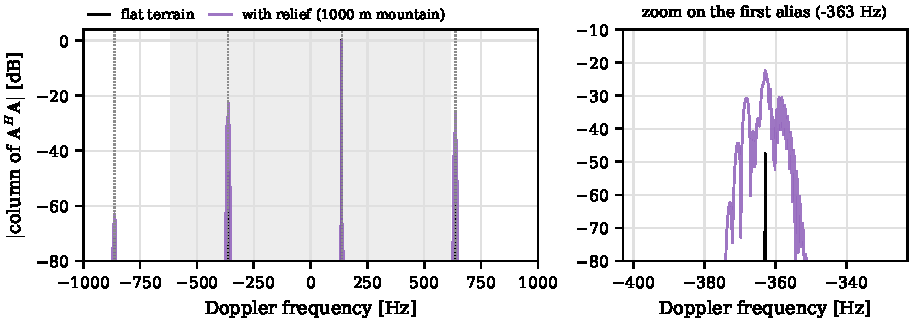
\includegraphics[width=\linewidth]{figures/system_coupling.pdf}
\caption[Coupling between Doppler bins in the joint model]{One column of $\mathbf A\Hm\mathbf A$ in the Doppler domain: the
response to a single Doppler bin of $g$ at \SI{137}{Hz}, for the formation of \cref{fig:example1d}, on flat terrain and with the
\SI{1000}{m} mountain. Dotted lines: the aliases of the bin, $\PRFop=\SI{500}{Hz}$ apart; grey: the processed band $\Ba$.
Right: zoom on the first alias.}
\label{fig:coupling}
\end{figure}

\subsection{The problem that is solved}

\begin{equation}
  \hat{\vg}=\arg\min_{\vg}\ \|\mathbf A\vg-\sv\|^2+\mu^2\|\vg\|^2
  \quad\Longleftrightarrow\quad
  \bigl(\mathbf A\Hm\mathbf A+\mu^2\mathbf I\bigr)\,\hat{\vg}=\mathbf A\Hm\sv ,
  \qquad \mu=0.03\,\sigma_{\max}(\mathbf A).
  \label{eq:tikhonov}
\end{equation}
The equivalence follows by setting the gradient of the cost to zero, $\mathbf A\Hm(\mathbf A\vg-\sv)+\mu^2\vg=\bm 0$.
$\sigma_{\max}$ is estimated by the power method, $\bm x\leftarrow\mathbf A\Hm\mathbf A\bm x/\|\mathbf A\Hm\mathbf A\bm x\|$
(12 iterations), $\sigma_{\max}\approx\sqrt{\|\mathbf A\Hm\mathbf A\bm x\|}$, which again uses only $\mathbf A$ and $\mathbf A\Hm$.

\paragraph{Why regularise ($\mu^2\|\vg\|^2$).} Writing $\mathbf A$ through its singular values,
$\mathbf A\bm v_k=\sigma_k\bm u_k$, every direction $\bm v_k$ of the scene is recovered with its own weight:
\begin{equation}
  \hat{\vg}=\sum_k \underbrace{\phi_k}_{\text{weight}}\,(\bm u_k\Hm\sv)\,\bm v_k ,
  \qquad
  \phi_k=\begin{cases}
    1/\sigma_k & \text{without $\mu$ (inverse)},\\[2pt]
    \dfrac{\sigma_k}{\sigma_k^2+\mu^2} & \text{with $\mu$ (Tikhonov)}.
  \end{cases}
  \label{eq:filterfactors}
\end{equation}
A small $\sigma_k$ is a direction that the channels hardly measure, for example parcels that the channels see with almost the
same phases (the conditioning discussed in \cref{sec:mismatch}). Without $\mu$, the factor $1/\sigma_k$ amplifies in those
directions the noise and the model errors (the echo shape that the model ignores, the interpolation of the height table,
rounding), and $\hat{\vg}$ explodes. With $\mu$: for $\sigma_k\gg\mu$, $\phi_k\approx1/\sigma_k$, the same as the inverse;
for $\sigma_k\ll\mu$, $\phi_k\approx\sigma_k/\mu^2\to0$, the direction is damped. With $\mu=0.03\,\sigma_{\max}$ only what the
channels measure with less than about \SI{3}{\percent} of the best direction is damped; the second pass recovers part of
what $\mu$ removed where the measurement is good.

\subsection{Conjugate gradients for least squares}

$\mathbf A\Hm\mathbf A+\mu^2\mathbf I$ is Hermitian and positive definite, so \eqref{eq:tikhonov} can be solved by conjugate
gradients. CGLS does it with products by $\mathbf A$ and $\mathbf A\Hm$ only, never forming the normal matrix (which would
also square the condition number in finite precision). The loop is in \cref{fig:flowline}:
\begin{itemize}
  \item each iteration costs one model ($\bm q=\mathbf A\bm p$) and one adjoint ($\bm z=\mathbf A\Hm\bm r-\mu^2\bm\delta$);
        $\alpha=\|\bm z\|^2/(\|\bm q\|^2+\mu^2\|\bm p\|^2)$ is the optimal step along the direction $\bm p$, and
        $\bm p\leftarrow\bm z+\beta\bm p$, $\beta=\|\bm z_{\mathrm{new}}\|^2/\|\bm z\|^2$, is conjugate to the previous
        directions, so no direction is searched twice;
  \item a pass stops when $\|\bm z\|\le10^{-4}\|\bm z_0\|$ or after 60 iterations, and adds its result to $\hat{\vg}$;
  \item two passes: the second solves the same problem for the residual left by the first and adds its solution to
        $\hat{\vg}$ (iterated Tikhonov). The weight becomes $\bigl[1-\bigl(\mu^2/(\sigma_k^2+\mu^2)\bigr)^2\bigr]/\sigma_k$,
        closer to $1/\sigma_k$ where the channels measure well and still zero where they do not;
  \item on the example of \cref{fig:example1d}: 120 iterations in total, with \SI{-40.3}{dB} of the channels left unexplained.
\end{itemize}

\subsection{The answer: \texorpdfstring{$U=K\odot\mathbf F\hat{\vg}$}{U = K F g}}\label{sec:joint-answer}

\paragraph{What is wanted.} The line that an ideal \emph{monostatic} radar, at the transmitter, would record at
$\PRF=\SI{2000}{Hz}$, without aliasing. In the simulation this is the reference. $\hat{\vg}$ is the scene; $U$ is that scene
recorded again by the ideal radar.

\paragraph{Where it comes from.} It is \caseref{3}, \eqref{eq:case3}, applied to the scene that was found:
\begin{equation}
  U(f)=\underbrace{K(f)}_{\text{echo of one point}}\ \underbrace{\hat G(f)}_{\mathcal F\{\hat{\gs}\}}
  \quad\Longleftrightarrow\quad
  u[n]=\sum_\ell \hat{\gs}[\ell]\,k[n-\ell],
  \label{eq:answer}
\end{equation}
i.e.\ one chirp at each position of the scene, weighted by $\hat{\gs}$ and summed.

\paragraph{Why without the screen.} The screen is the phase of channel $i$ \emph{relative to the monostatic} path; for the
monostatic radar itself it is one ($\bat=\bxt=0\Rightarrow C_0=0\Rightarrow\Delta C_0=0\Rightarrow\theta\equiv1$). The
effects of the topography are therefore split as in \cref{tab:topo}: the monostatic phase of each target is common to all
channels and is part of its amplitude $a_p$, so it is estimated inside $\hat{\vg}$ and reaches $U$, exactly as in the
reference; the channel-dependent phase lives in the model $\mathbf A$ and is used only to explain the channels. $U$ thus
contains what the reference contains, the scene with its monostatic phases, and none of the phases that differ between
channels, which are the ones that create the ambiguities.

\begin{table}[htbp]
\centering
\caption[How the topography enters the joint model]{How each effect of the topography enters the joint model and the answer $U$.}
\label{tab:topo}
\footnotesize\setlength{\tabcolsep}{4pt}
\begin{tabular}{@{}>{\raggedright\arraybackslash}p{43mm}>{\raggedright\arraybackslash}p{38mm}>{\raggedright\arraybackslash}p{30mm}>{\raggedright\arraybackslash}p{20mm}@{}}
\toprule
effect of the topography & type & in the model & in $U$? \\
\midrule
monostatic range phase, $\e^{-\jj4\pi r_p/\lambda}$ & constant per target, same in every channel & in $a_p$ (inside $\vg$) & yes, through $\hat{\vg}$ \\
extra phase of channel $i$, $\varphi_i=2\pi\Delta C_{0,i}/\lambda$ & constant per target, differs per channel & screen $\theta_i$ (inside $\mathbf A$) & no ($\theta\equiv1$) \\
echo shape ($K_a\propto1/r$; $C_1$, $C_2$ with $h$) & not constant & ignored ($\Delta r/r\approx\SI{0.1}{\percent}$) & --- \\
\bottomrule
\end{tabular}
\end{table}

\paragraph{Why back to the raw line, and not stop at $\hat{\vg}$.}
\begin{itemize}
  \item \emph{Fair comparison:} the reference, the standard reconstruction, SATA and the joint reconstruction all return the
        raw line of $12288$ samples at \SI{2000}{Hz}; the focusing that follows is the same for all of them.
  \item \emph{Band:} outside $|f|\le\Ba/2$ the data do not determine $\vg$; the multiplication by $K$ and the band cut
        discard that part.
  \item \emph{SAR chain:} the reconstruction is a pre-processing step (aliased channels in, one clean channel out); the SAR
        processor expects raw data.
\end{itemize}
In practice $U=K\odot\mathbf F\hat{\vg}$, then $U(f)=0$ for $|f|>\Ba/2$ ($\Ba=\SI{1234.8}{Hz}$), and the line is
$\mathbf F^{-1}U$, in the same format as the standard reconstruction.

\paragraph{Afterwards (the same for every method).} The focusing is
$\text{image}=\mathbf F^{-1}\{K^*U\}=\mathbf F^{-1}\{|K|^2\hat G\}$, i.e.\ $\hat G$ with a smooth window inside the band: one
peak per target ($\SI{-3}{dB}$ width $\approx\SI{5.8}{m}$). The metric of \cref{sec:metric} is then the highest ghost at the
folds relative to the peak of the reference. \Cref{fig:answer} summarises the chain.

\begin{figure}[htbp]
\centering
% From the channels to the image: inversion, re-recording, focusing
\begin{tikzpicture}[x=1cm,y=1cm]
  \node[blk,draw=cblue,fill=cblue!8,text width=22mm] (s) at (0,0) {$\textcolor{cblue}{\bm s}$\\[1pt] \footnotesize $\Nrx=4$ channels\\ \footnotesize \SI{500}{Hz}, aliased};
  \node[blk,draw=cred,fill=cred!6,text width=22mm] (g) at (4.5,0) {$\textcolor{cred}{\hat{\bm g}}$\\[1pt] \footnotesize the scene\\ \footnotesize (peaks at targets)};
  \node[blk,draw=caqua!80!black,fill=caqua!10,text width=22mm] (U) at (9.0,0) {$U$\\[1pt] \footnotesize 1 channel, \SI{2000}{Hz}\\ \footnotesize no aliasing};
  \node[bdata,text width=19mm] (im) at (13.2,0) {image\\[1pt] \footnotesize dB at the folds};
  \draw[seta] (s) -- node[above=1pt,nota]{invert $\mathbf A$\\ (CGLS)} (g);
  \draw[seta] (g) -- node[above=1pt,nota]{re-record:\\ $\times K$,\\ band cut} (U);
  \draw[seta] (U) -- node[above=1pt,nota]{focus:\\ $\times K^{*}$} (im);
  \node[bdata,text width=40mm] (ref) at (9.0,-2.1) {reference (simulated directly)};
  \draw[seta,dashed] (ref) -- node[right,nota]{$U\approx$ reference} (U);
  \node[nota,anchor=north] at (6.6,-2.85) {example: reference \SI{-48.7}{dB}\qquad joint reconstruction \SI{-43.5}{dB}\qquad no SATA \SI{-8.7}{dB}};
\end{tikzpicture}

\caption[From the channels to the image]{From the aliased channels to the image. The joint reconstruction inverts the model to
find the scene $\hat{\vg}$, records it again with the ideal monostatic radar ($\times K$ and band cut) to obtain $U$, which is
compared with the reference simulated directly; the focusing is the same for every method. Values: example of
\cref{fig:example1d}.}
\label{fig:answer}
\end{figure}

\section{Properties}

\begin{itemize}
  \item \textbf{Consistency.} With a zero DEM the method reproduces the standard reconstruction within \SI{0.1}{\percent} rms.
  \item \textbf{Information used.} Only the channels, the system geometry and the DEM. The positions of the targets are never
        used (\cref{sec:sata-maps}).
  \item \textbf{Self-test of the DEM.} The part of the channels that the model does not explain is \SIrange{-41}{-39}{dB} with
        the right DEM and \SIrange{-20}{-7}{dB} with a wrong one (mirrored or shifted by \SI{1}{km}), which makes it a natural
        alarm for DEM errors.
  \item \textbf{Cost.} About \SI{3.3}{s} per line with four channels in the 1-D simulator (median over 680 runs), against
        \SI{0.15}{s} for SATA whole band.
  \item \textbf{Convergence.} \Cref{fig:convergence} follows the iterations on the example of \cref{fig:example1d}. The
        first iteration is the adjoint, i.e.\ the channels focused, corrected and summed (\SI{-10.2}{dB}, close to no SATA);
        about ten iterations bring the ambiguities below \SI{-39}{dB}, and the second pass gains another \SI{1}{dB}
        (\SI{-43.5}{dB} after $2\times60$ iterations). The unexplained part of the channels falls to \SI{-38}{dB} in the same
        way.
  \item \textbf{Ill-conditioned configurations.} Where the baselines do not separate the parcels (two channels, equally
        spaced baselines, certain heights with long baselines) the information is not in the data; the regularisation then
        leaves the ambiguity instead of amplifying noise.
\end{itemize}

\begin{figure}[htbp]
\centering
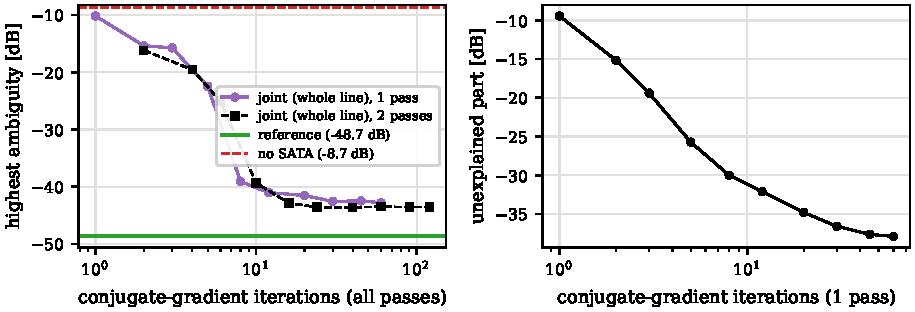
\includegraphics[width=\linewidth]{figures/joint_convergence.pdf}
\caption[Convergence of the joint reconstruction]{Joint reconstruction over the whole line on the example of
\cref{fig:example1d} (five targets on a \SI{1000}{m} mountain, four channels). Left: highest ambiguity against the total number of
conjugate-gradient iterations, with one pass and with two passes, against the reference and no SATA. Right: part of the channels
that the model does not explain, $\|\bm s-\mathbf A\hat{\bm g}\|/\|\bm s\|$, during the first pass.}
\label{fig:convergence}
\end{figure}

\Cref{fig:example1d} shows the example used throughout the development: five targets on a \SI{1000}{m} Gaussian mountain
with $\bxt=[0,134.9,20.5,8.3]$\,\si{m}. The highest ambiguity goes from \SI{-8.7}{dB} without correction to \SI{-43.5}{dB}
with the joint reconstruction; the reference is \SI{-48.7}{dB}, and \SI{-43.9}{dB} once it is limited to the processed band
$\Ba$, as every reconstruction is.

\begin{figure}[p]
\centering
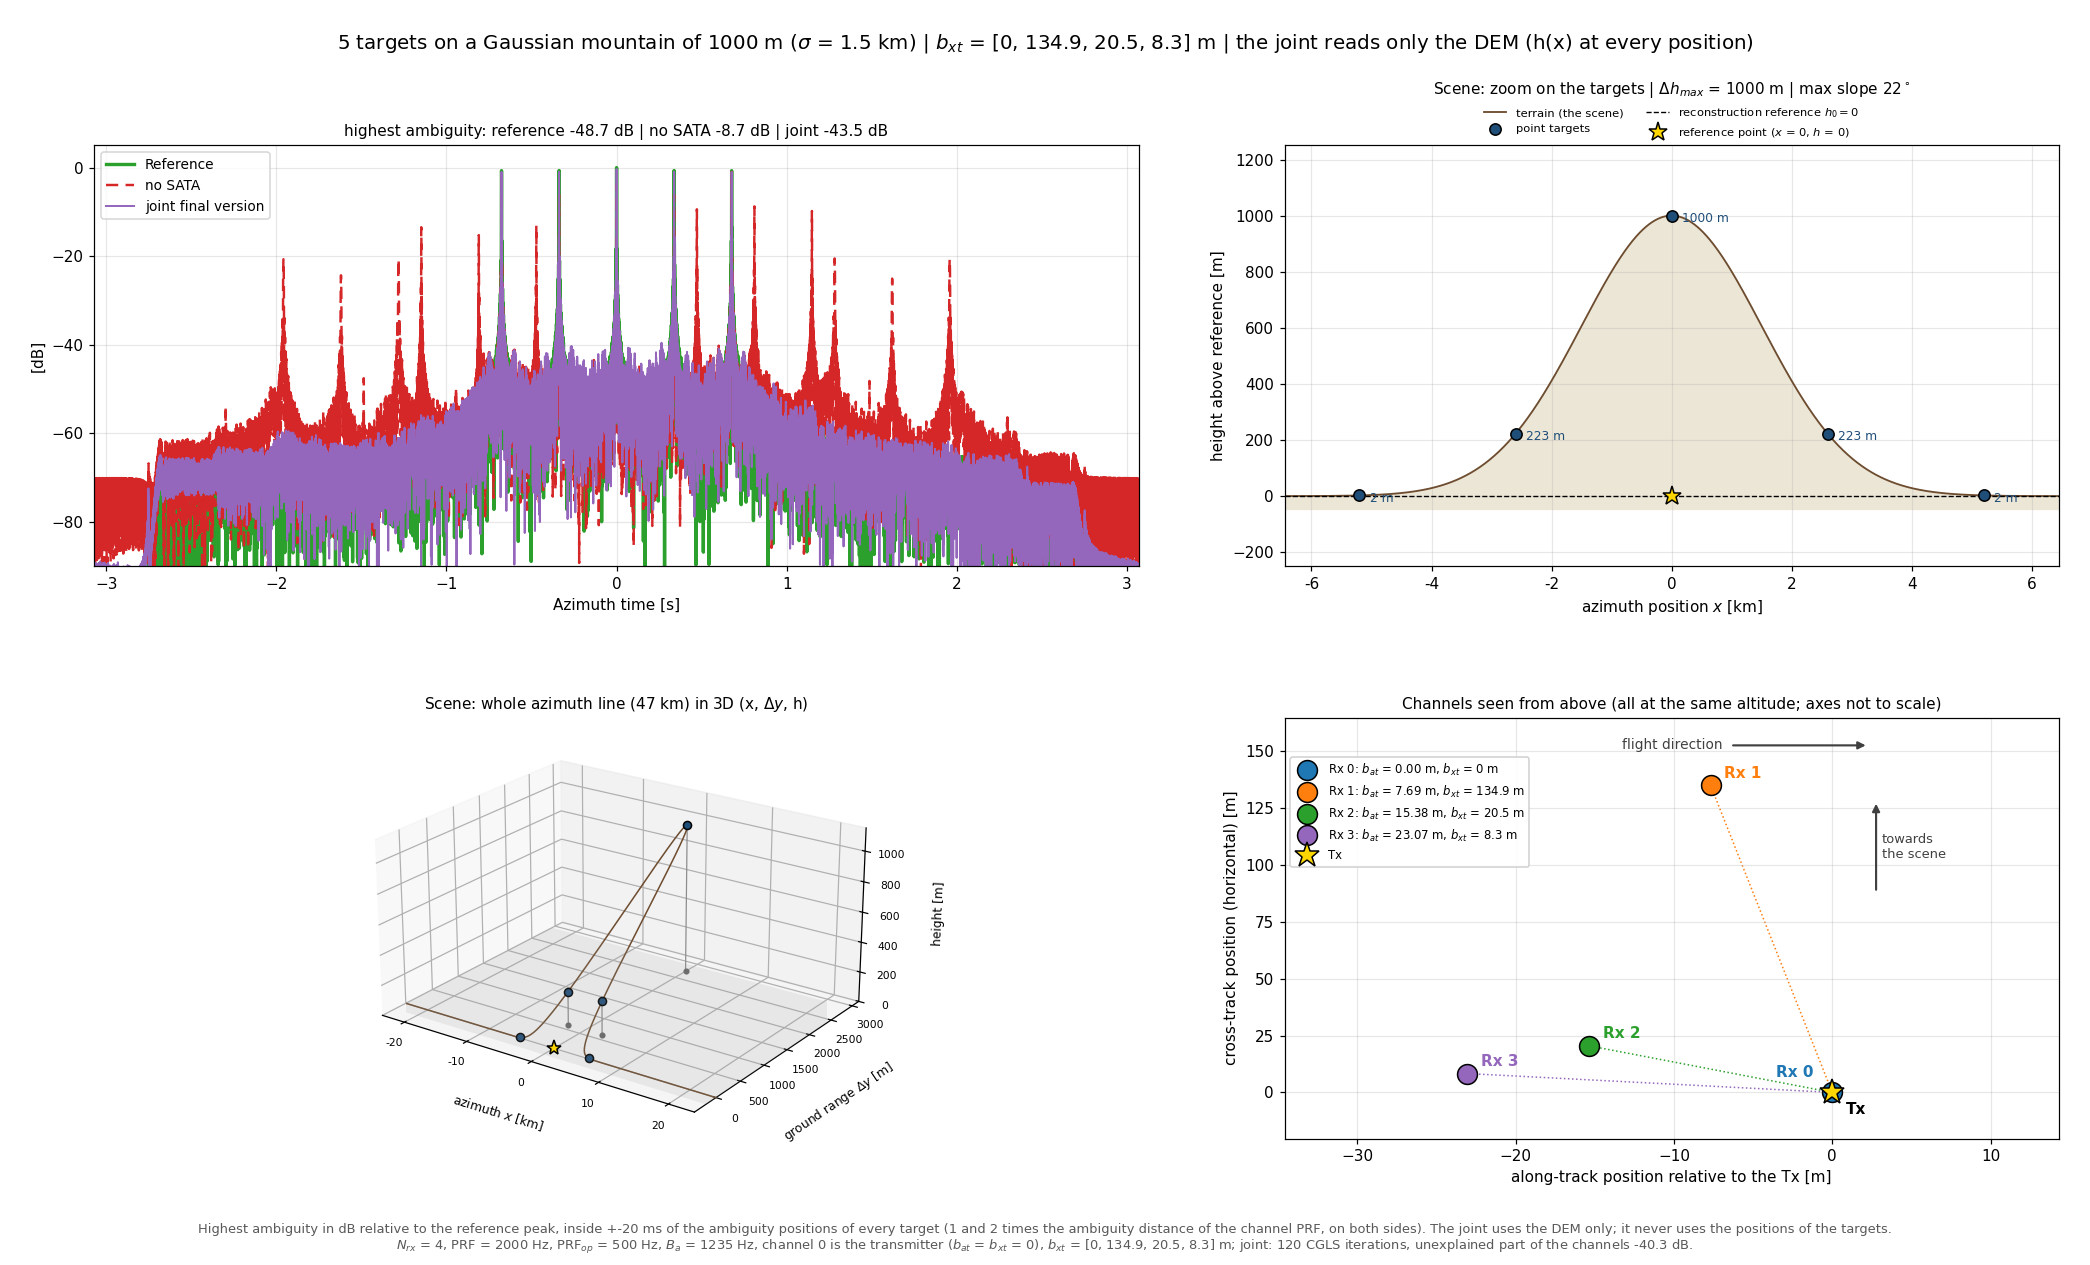
\includegraphics[width=\linewidth]{figures/joint_example_1d.png}
\caption[Example: five targets on a mountain]{Five targets on a \SI{1000}{m} Gaussian mountain, four channels. Top left:
azimuth impulse responses of the reference, of the standard reconstruction (no SATA) and of the joint reconstruction over the
whole line. Right: the scene and the formation. The joint reconstruction reads only the DEM.}
\label{fig:example1d}
\end{figure}
